% !TeX spellcheck = it_IT
\section{Comunicazione Wireless}
Tutte le comunicazioni nel mondo wired avvengono tipicamente in banda base, i.e., data una banda $B$ trasmetto direttamente usando lo spettro di frequenze $[0,B]$.\\ 

Problemi:
\begin{enumerate}
	\item Se tutti i dispositivi trasmettessero in banda base, tutte le comunicazioni radio farebbero interferenza l'una con l'altra
	\item Più è bassa la frequenza più grande deve essere l'antenna ($\lambda/2$ per antenna dipole, es: $1MHz \sim 142$ metri, $2100MHz \sim 7$ cm)
	\item Ogni range di radio frequenze possiede diverse proprietà i propagazione e attenuazione
\end{enumerate}

\paragraph{Spettro elettromagnetico per le telecomunicazioni:}
\begin{center}
	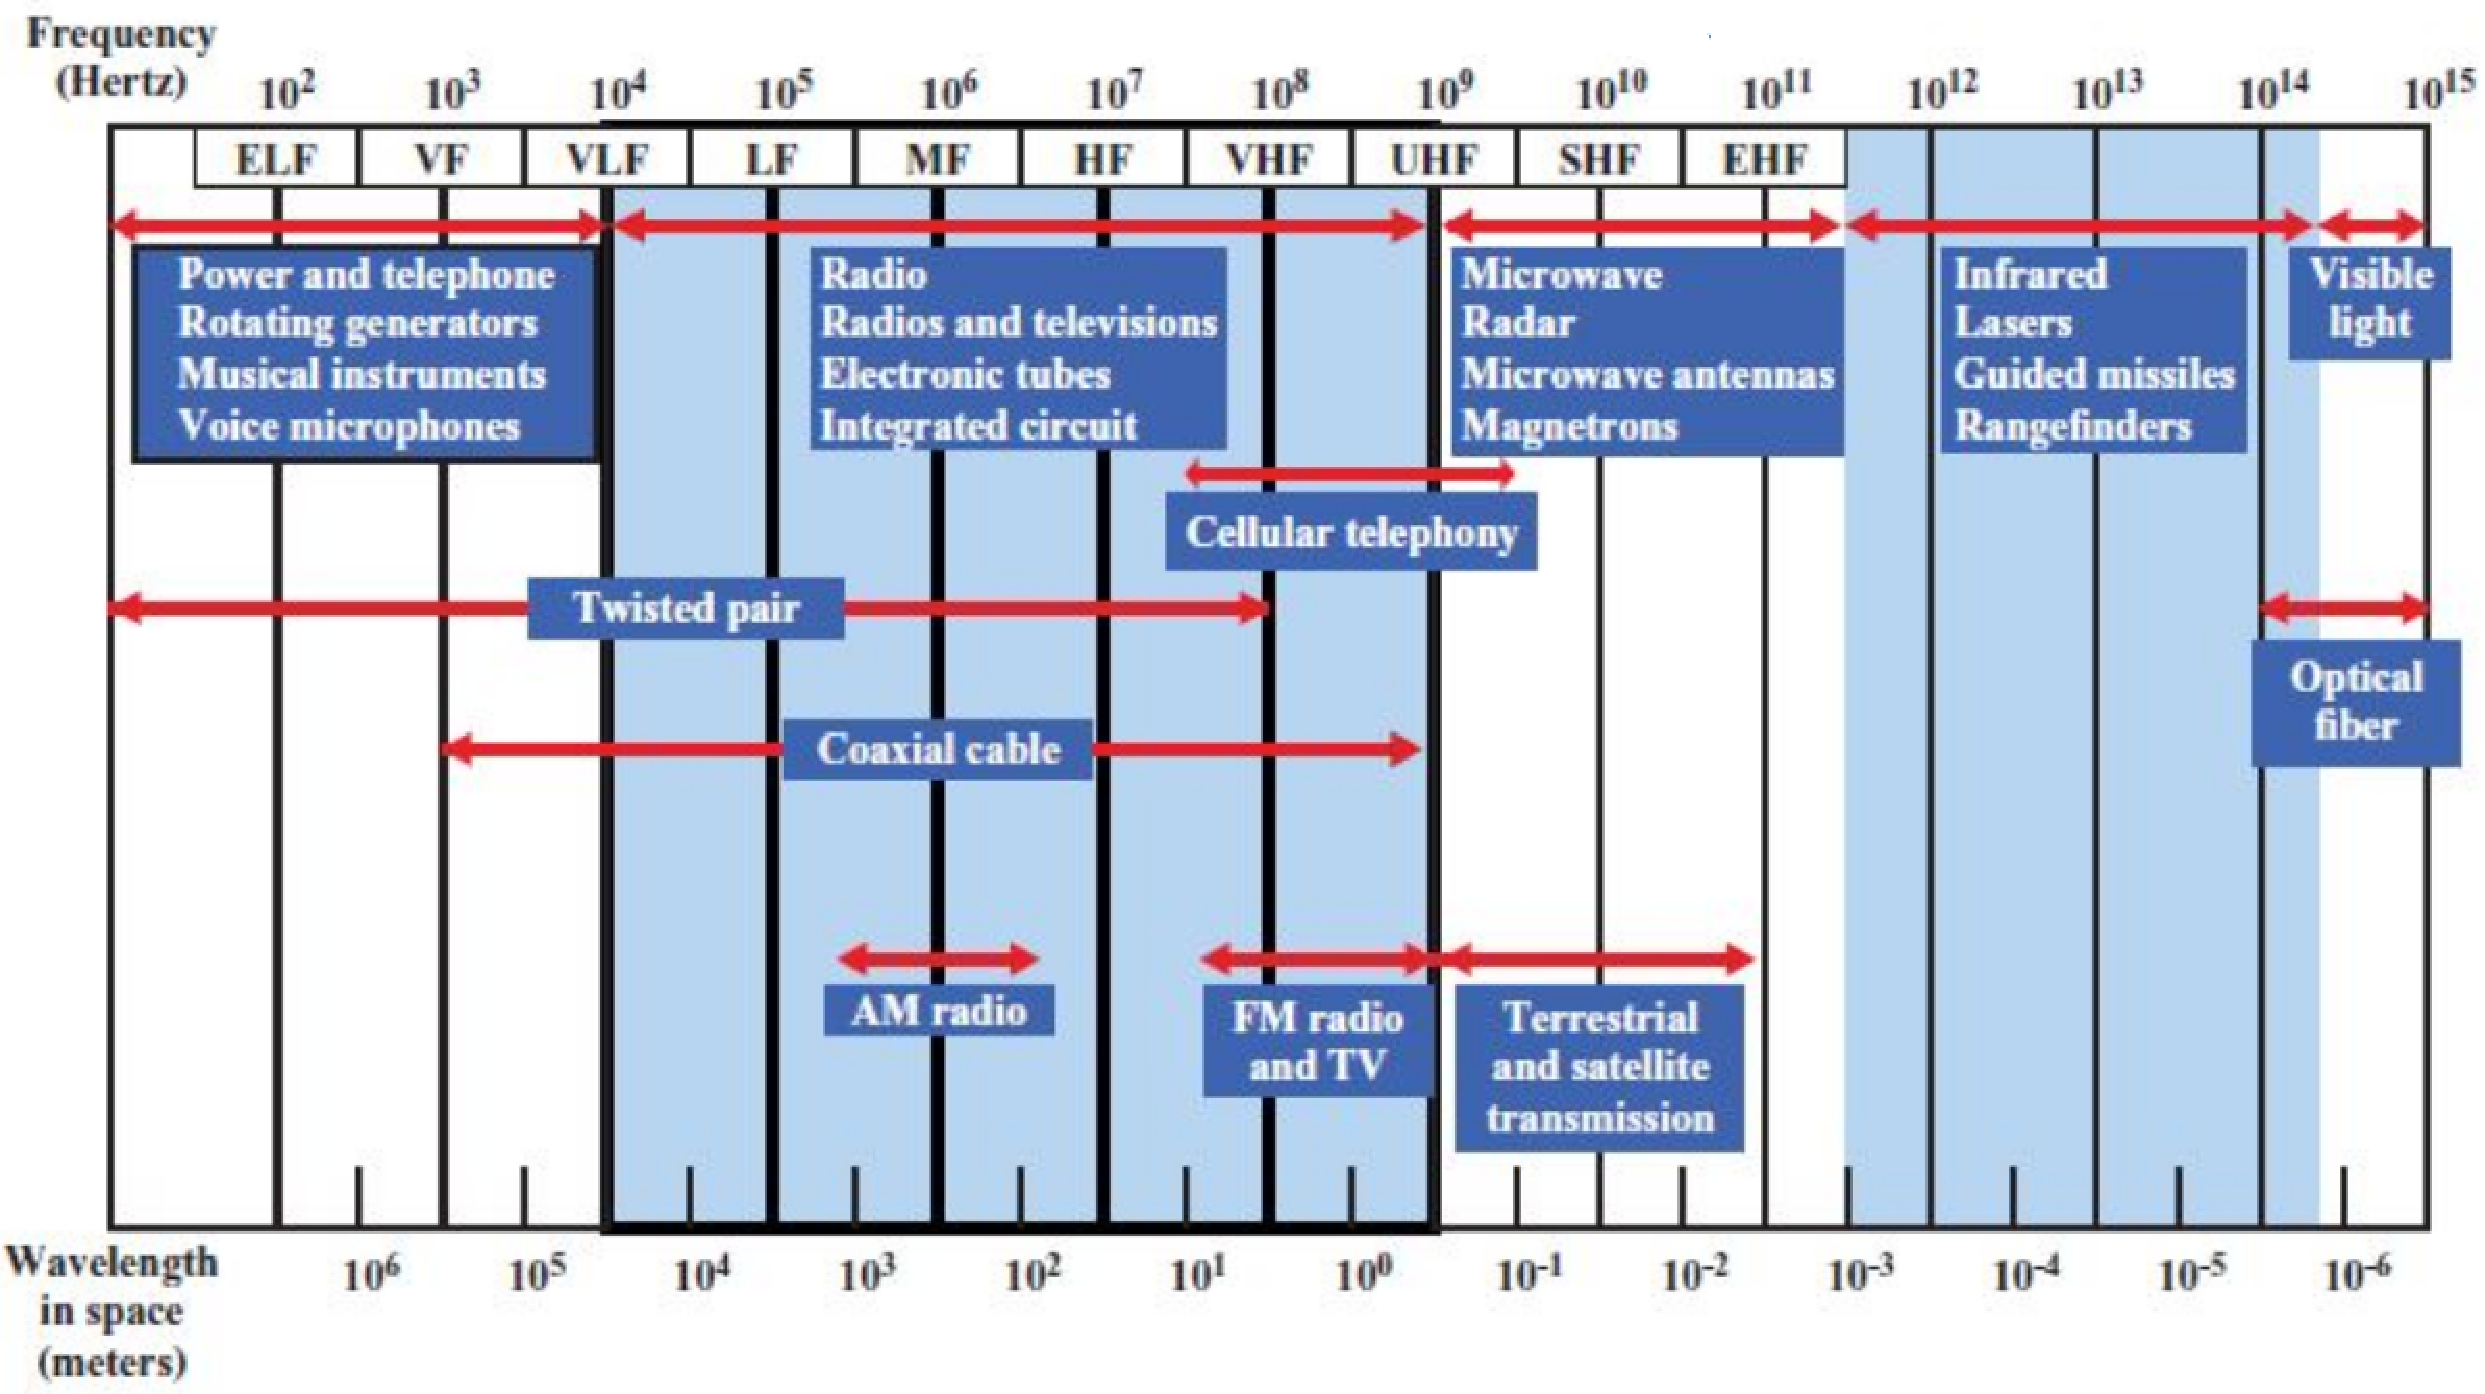
\includegraphics[width=0.98\linewidth]{img/wireless/emspectrum1}
\end{center}
Molto approssimativo, c'è uno standard per ogni tipo di telecomunicazione (\href{https://upload.wikimedia.org/wikipedia/commons/thumb/c/c7/United_States_Frequency_Allocations_Chart_2016_-_The_Radio_Spectrum.pdf/page1-1200px-United_States_Frequency_Allocations_Chart_2016_-_The_Radio_Spectrum.pdf.jpg}{\texttt{allocazione delle frequenze per gli USA}}).\\

\newpage

\paragraph{Trasmissione in banda traslata:} Da $[0,B]$ spostiamo la banda all'interno di un altro range, ovvero $[f_c - B/2, f_c + B/2]$, la stessa banda ma traslata attorno ad una frequenza portante $f_c$.
\begin{center}
	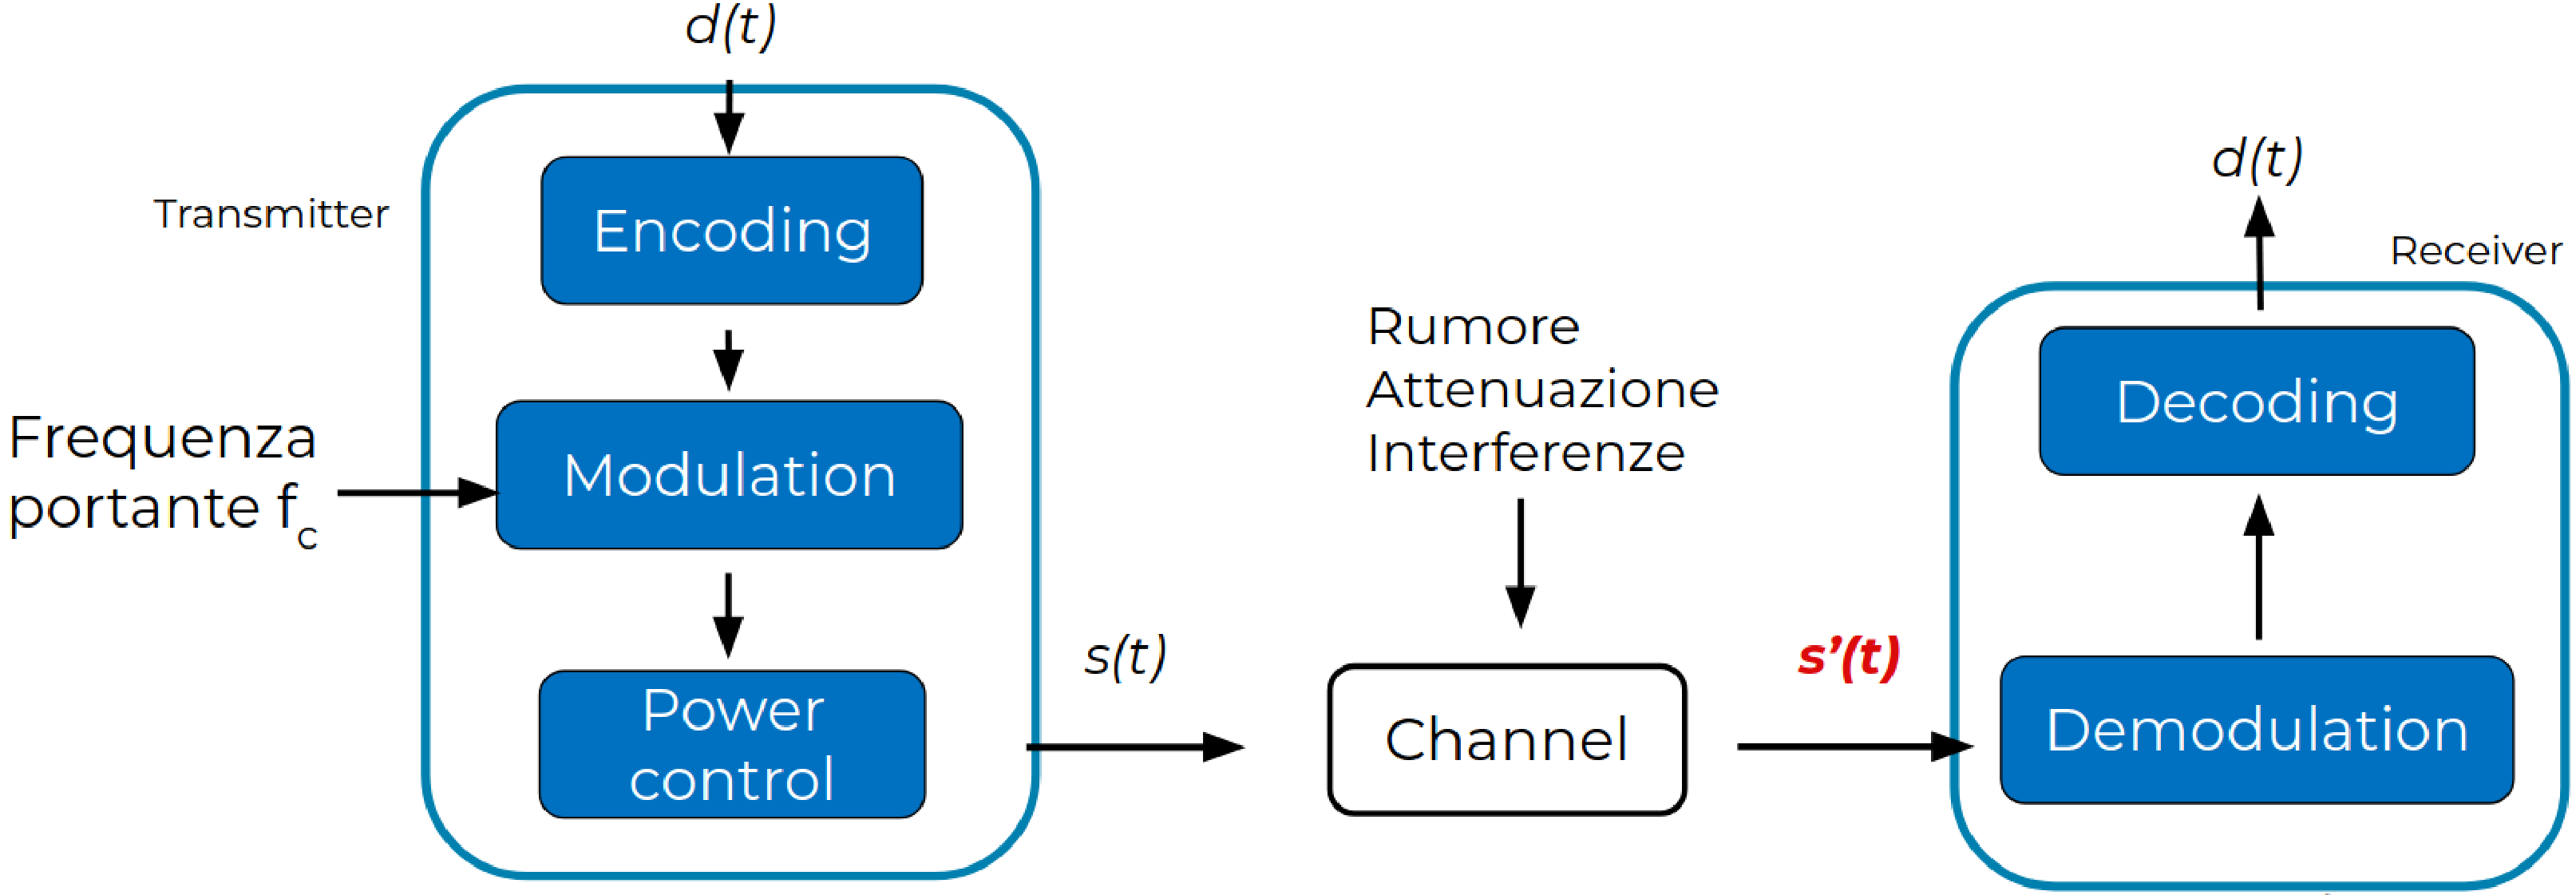
\includegraphics[width=0.95\linewidth]{img/wireless/bandatraslata1}
\end{center}
Il compito del trasmettitore diventa codificare, \textbf{modulare attorno alla frequenza portante} $f_c$ ed il trasmettitore deve de-modulare, pulire e decodificare il segnale trasmesso. Bandwidth e data rate rimangono gli stessi, cambia solo "dov'è" la banda.\\

Domande: 
\begin{enumerate}
	\item Che spettro utilizzare? (che frequenza portante scegliere)
	\item Come codifico i dati? (da digitale ad analogico)
	\item Come modulo il mio segnale in banda base sulla frequenza portante?
\end{enumerate}

\newpage

\subsection{Encoding, symbol e symbol rate}

\paragraph{Simbolo:} Una forma d'onda, uno stato o una condizione significativa del canale di comunicazione che persiste per un intervallo di tempo fissato. Esempio: voltaggio a $3V$ per 1 secondo.\\

\paragraph{Symbol rate:} Quantità di simboli trasmessi al secondo (misurato in baud). Dipende dal processore fisico.\\

In generale, un \textbf{simbolo può contenere più bit} (codifica e modulazione), quindi \textbf{symbol rate $\neq$ bit rate}.\\
Generalmente, più la distanza da coprire si allunga più la durata si abbassa.\\

Una data bandwidth può supportare diversi data rate, a seconda dell'abilità del ricevente di distinguere 0 e 1 in presenza di rumore.\\

Possiamo codificare tramite una modulazione in ampiezza: data una entry di bit scegliamo il voltaggio corrispondente
\begin{center}
	\includegraphics[width=\linewidth]{img/wireless/modam1}
\end{center}
Moduliamo la portante (modifichiamo l'ampiezza) in base ai bit da codificare. Usato nelle radio AM. Si può vedere che symbol rate e data rate sono diversi, ogni simbolo (livello di ampiezza) rappresenta due bit.\\

\newpage

\subsection{Trasmissione delle onde radio}

\paragraph{Propagazione onde radio:} Ci sono più possibili tipi di propagazione delle onde radio, in base alla frequenza utilizzata
\begin{itemize}
	\item Ground Wave Propagatio (sotto i $2MHz$): il segnale segue la curvatura della terra
	\item Sky Wave Propagation (da $2$ a $30MHz$): il segnale rimbalza nella ionosfera
	\item \textbf{Line of sight LOS} (sopra $30MHz$): Deve esserci una linea diretta (anche non a vista in realtà, ma diretta) tra trasmettitore e ricevitore
\end{itemize}

\paragraph{Tipi di antenne:}
\begin{itemize}
	\item Omnidirezionale (a sinistra), la potenza emessa è uguale in tutte le direzioni (ideale)
	\item Direzionale (a destra): si vuole propagare segnale in una sola direzione, non ideale, ma solitamente la propagazione non è limitata strettamente ad una direzione
\end{itemize}
\begin{center}
	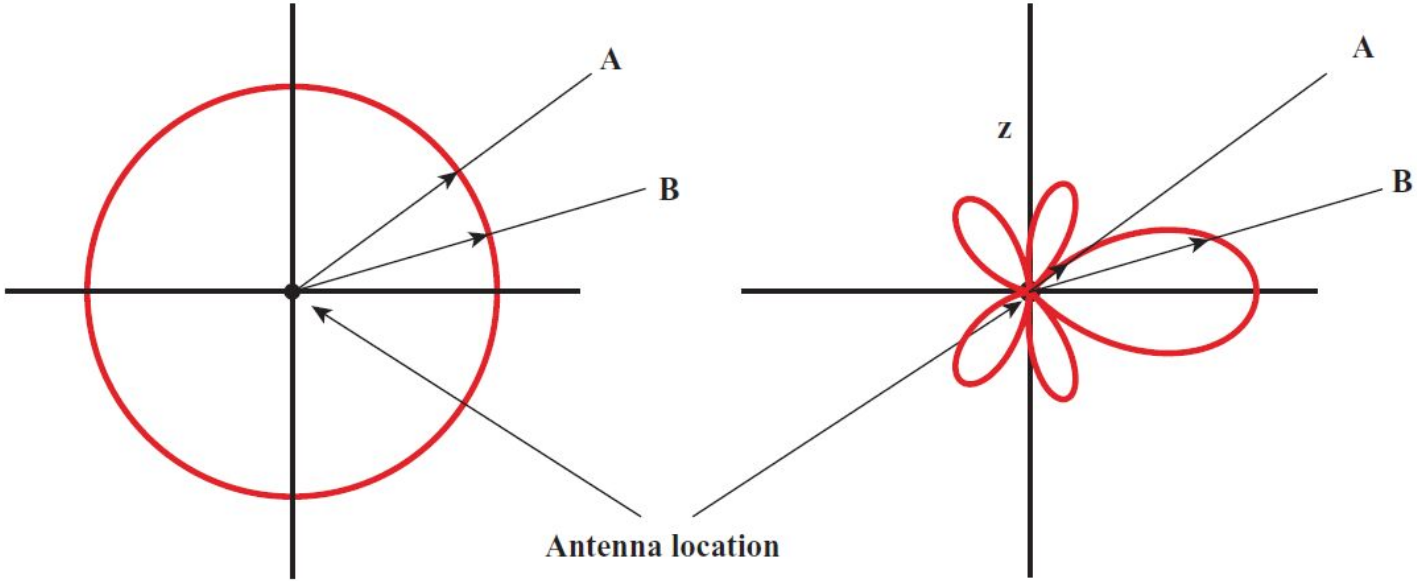
\includegraphics[width=0.9\linewidth]{img/wireless/antenna}
\end{center}

\newpage

\subsubsection{Problemi con Trasmissione radio Line of Sight (LOS)}

Ci sono problemi legati alla trasmissione LOS:
\begin{itemize}
	\item Free space loss \& path loss: attenuazione del segnale dovuta alla distanza e all'ambiente in cui il segnale si propaga; cosa perdo da antenna trasmettitrice (TX) a ricevitrice (RX)
	\item Rumore: disturbo che può distorcere il segnale
	\item Multipath: il segnale tra TX e RX può subire riflessioni, diffrazioni e scattering causando la ricezione di più onde elettromagnetiche dello stesso segnale in tempi diversi; per qualche motivo, un riflesso del segnale giunge al ricevitore, in momenti diversi dall'originale, possono diventare interferenze per segnali successivi
	\item Effetto Doppler: Il segnale cambia a causa del movimento di RT, TX e ostacoli; il segnale ricevuto potrebbe essere su una frequenza "vicina" a quella originale, disturbando la fingerprint di un segnale
\end{itemize}

\paragraph{Path Loss:} Attenuazione del segnale radio in funzione della distanza tra trasmettitore e ricevitore.
$$ \frac{P_t}{P_r} = \left(\frac{4 \pi}{\lambda}\right)^2 d^n = \left(\frac{4 \pi f}{c}\right)^2 d^n $$
Misurata in $dB$, rapporto tra potenza del segnale trasmesso (fisso) rispetto alla potenza del segnale ricevuto (diventa sempre più piccolo, in base alla distanza).\\

Direttamente proporzionale (al quadrato della) alla frequenza, direttamente proporzionale ad una potenza della distanza, l'esponente $n$ dipende dall'ambiente (più l'ambiente è ostruito più la distanza sarà influente).\\

%End L2